% README.tex — PCB-Wish 桌面版使用说明
% 编译：在仓库根目录运行
%   xelatex -output-directory=docs/readme/build README.tex
% 连跑 3 次，让目录和页码收敛。
\documentclass[11pt,a4paper]{ctexart}

% ---------- 字体 ----------
\setCJKmainfont[AutoFakeBold=2.5]{SimSun}
\setCJKsansfont[AutoFakeBold=2.5]{SimHei}
\setCJKmonofont{SimSun}

% ---------- 页面与颜色 ----------
\usepackage[a4paper,left=2.3cm,right=2.3cm,top=2.5cm,bottom=2.4cm,headheight=22pt]{geometry}
\usepackage[table]{xcolor}
\definecolor{ink}{HTML}{2F3631}
\definecolor{ink2}{HTML}{6C7269}
\definecolor{sage}{HTML}{6B7E72}
\definecolor{sagedark}{HTML}{4F5F55}
\definecolor{copper}{HTML}{A9825F}
\definecolor{cream}{HTML}{F7F5F0}
\definecolor{line}{HTML}{DED9CD}
\definecolor{brick}{HTML}{A9605A}
\definecolor{okbg}{HTML}{ECEFEB}

\usepackage{graphicx}
\usepackage{booktabs}
\usepackage{tabularx}
\usepackage{array}
\usepackage{ragged2e}
\usepackage{enumitem}
\usepackage{amsmath}
\usepackage{amssymb}
\usepackage{caption}
\usepackage{fancyhdr}
\usepackage{tikz}
\usetikzlibrary{arrows.meta,positioning}
\usepackage[most]{tcolorbox}
\usepackage{hyperref}

\graphicspath{{docs/readme/images/}}

% ---------- 基本排版 ----------
\linespread{1.25}
\setlength{\parindent}{0pt}
\setlength{\parskip}{0.5em}
\setlength{\emergencystretch}{3em}
\RaggedRight
\setlength{\tabcolsep}{5pt}
\renewcommand{\arraystretch}{1.24}
\setcounter{tocdepth}{1}
\setcounter{secnumdepth}{2}

\ctexset{
  section/format={\Large\bfseries\color{sagedark}},
  subsection/format={\large\bfseries\color{ink}},
  subsubsection/format={\normalsize\bfseries\color{ink}},
}

\captionsetup{
  font=small,
  labelfont={bf,color=sagedark},
  labelsep=quad,
  justification=centering,
  skip=6pt
}

\hypersetup{
  colorlinks=true,
  linkcolor=sagedark,
  urlcolor=copper,
  pdftitle={PCB-Wish 桌面版使用说明},
  pdfauthor={PCB-Wish Project},
  pdfsubject={从自然语言需求到可制造 PCB 的智能设计系统}
}
\urlstyle{same}

% ---------- 页眉页脚 ----------
\pagestyle{fancy}
\fancyhf{}
\fancyhead[L]{\small\color{ink2}PCB-Wish 桌面版 · 使用说明}
\fancyhead[R]{\small\color{ink2}\thepage}
\renewcommand{\headrulewidth}{0.4pt}
\renewcommand{\headrule}{\hbox to\headwidth{\color{line}\leaders\hrule height \headrulewidth\hfill}}

% ---------- 小工具 ----------
\newcommand{\code}[1]{\texttt{\small #1}}

\newtcolorbox{leadbox}{
  enhanced,
  colback=cream,
  colframe=copper,
  boxrule=0.6pt,
  arc=1.5mm,
  left=5mm,right=5mm,top=3.5mm,bottom=3.5mm
}

\newtcolorbox{warnbox}{
  enhanced,
  colback=brick!4,
  colframe=brick!75,
  boxrule=0.6pt,
  arc=1.5mm,
  left=5mm,right=5mm,top=3.5mm,bottom=3.5mm
}

\newtcolorbox{notebox}{
  enhanced,
  colback=okbg,
  colframe=sage!65,
  boxrule=0.5pt,
  arc=1.5mm,
  left=5mm,right=5mm,top=3mm,bottom=3mm
}

\setlist[itemize]{leftmargin=1.4em,itemsep=0.24em,topsep=0.22em}
\setlist[enumerate]{leftmargin=1.7em,itemsep=0.24em,topsep=0.22em}

\begin{document}

% ==================== 封面 ====================
\begin{titlepage}
\thispagestyle{empty}
\centering
\vspace*{1.0cm}


\includegraphics[width=1.5cm]{app-icon.png}\\[0.8cm]
{\color{sage}\rule{0.74\textwidth}{1pt}}\\[0.8cm]

{\Huge\bfseries\color{ink} PCB-Wish 桌面版}\\[0.4cm]
{\LARGE\color{sagedark} 从自然语言需求到可制造 PCB}\\[0.35cm]
{\large\color{ink2} 使用说明 · 工作流程 · 测试报告}\\[0.6cm]
{\color{copper}\rule{0.74\textwidth}{0.5pt}}\\[0.9cm]

\begin{minipage}{0.80\textwidth}
\RaggedRight
\large\color{ink}
本文说明 PCB-Wish 桌面版的功能、使用方式、系统流程与测试结果。
\end{minipage}\\[0.9cm]

\vfill
{\small\color{ink2} 版本 3.16.2 ｜ 2026 年 10 月 ｜ Windows 10/11 64 位}
\end{titlepage}

% ==================== 目录 ====================
\newpage
\thispagestyle{empty}
\tableofcontents
\vfill
{\small\color{ink2} 建议阅读顺序：文首了解创作背景；第 4、5 节了解使用方式；第 6 节了解系统流程；第 7、8 节了解边界与测试结果。}
\newpage
\pagenumbering{arabic}

% ==================== 创作背景 ====================
\section*{创作背景}
\addcontentsline{toc}{section}{创作背景}

PCB-Wish 是一个面向 PCB 设计的桌面智能体系统：用户用自然语言描述一块绘制难度不大的目标板卡，agent 系统通过分阶段工作完成需求澄清、选型、原理图与 PCB 绘制和检查验证，并导出可交付制造的工程文件；用户显式要求时还会生成配套教学讲义。本项目的板卡设计与交付流程全部使用国产生产工具：桌面端基于 ZCode 的开源框架进行任务特化的修改，设计执行使用嘉立创EDA专业版。

它的灵感来源于工科创课程的教学全过程。工科创课程中已经涉及电子设计、板卡绘制等内容，但无法覆盖每个人的需求和兴趣。

笔者更希望它成为一个兴趣驱动的学习工具，让同系大多数同学在修读工科创、并具备一定电子基础后，能够借助大模型工具完整尝试制作一块自己感兴趣功能的板卡，并在项目过程中学习电子设计的数值计算、元器件选型等方法，自主进行项目式学习。

笔者受此启发，希望借助当下发展迅速的大模型，把电子设计学习与同学们感兴趣的项目结合起来。通过开发这个 agent，既希望帮助同学们把设计想法落地，也希望通过随附讲义辅助同学们完成学习。系统工作流来源于笔者完整的打板流程，项目也尝试把“AI+教与学”落在这一过程中。

% ==================== 1 ====================
\section{项目概述}

PCB-Wish 将自然语言硬件需求转化为可制造的 PCB 工程。用户描述目标板卡，系统完成需求澄清、器件选型、原理图设计、PCB 布局布线、检查验证，最终输出 Gerber、钻孔、BOM、贴片坐标和检查报告。教学讲义不是默认交付物；用户在受理时用显式语言要求后，系统才会在制造文件完成后生成一份 LaTeX 排版的 PDF 讲义。

嘉立创是国产 PCB 平台，其 EDA 的适用范围正是本项目的甜区；生态涵盖开源社区与立创商城，可一站式打板。agent 全量接入其官方商城 API 与 EDA API，从立创商城选型，到嘉立创EDA 中绘制原理图、PCB 与布线，覆盖从选型到制造文件的全栈工作。ZCode 作为国产开源项目，其完善的 agent 框架使开发更快捷便利；原生环境与用户交互结合嘉立创生态，实现了基础的“许愿式开发”。

系统由受理、选型、设计、质检等角色协同工作，讲义作者在项目需要教学讲义时介入。受理角色负责把需求整理为可验收的规格；设计角色负责选型、画图与布线；质检角色独立复核设计结果。

\begin{center}
\small
\begin{tabularx}{\linewidth}{@{}>{\bfseries}p{3.6cm} >{\RaggedRight\arraybackslash}X@{}}
\toprule
\rowcolor{okbg}输入 & 输出 \\
\midrule
自然语言需求 & 需求说明书 \code{MISSION.md} \\
数据手册、旧图、照片 & 选型结果与 BOM \\
尺寸、成本、工艺约束 & 原理图、PCB、布线、铺铜、丝印 \\
关键问题答复 & Gerber、钻孔、BOM、贴片坐标 \\
显式要求“教学讲义” & LaTeX 源码与 PDF 讲义 \\
\bottomrule
\end{tabularx}
\end{center}

% ==================== 2 ====================
\section{适用范围}

系统当前面向 2 层或 4 层的低速数字与模拟板卡，适合传感器板、转接板、电源小板、模块底板和开发板周边。典型场景包括课程设计、实验室项目、小批量打样和需要同步产出教学资料的设计任务。

系统按阶段管理设计范围：需求评审阶段会检查层数、信号类型、工艺与装配方式；超出当前能力范围时，系统会建议简化、降速或分期，并在需求说明书中记录。

% ==================== 3 ====================
\section{环境要求}

\begin{center}
\small
\begin{tabularx}{\linewidth}{@{}>{\bfseries}p{4.0cm} >{\centering\arraybackslash}p{1.4cm} >{\RaggedRight\arraybackslash}X@{}}
\toprule
\rowcolor{okbg}项目 & 要求 & 说明 \\
\midrule
操作系统 & 必需 & Windows 10/11 64 位；其他系统可从源码构建，验证仍在进行。\\
嘉立创EDA专业版 & 必需 & 版本 $\ge$ 4.1.60；用于画图、检查与制造文件导出。\\
Python & 必需 & 3.10 或更新；插件脚本依赖。安装时加入 PATH。\\
大模型 API Key & 必需 & 兼容 OpenAI 接口；支持工具调用；上下文建议 1M。\\
xelatex & 可选 & 生成教学讲义 PDF 时使用。\\
ngspice & 可选 & 电路仿真；缺失时相关检查标记为“未执行”。\\
freerouting & 可选 & 密集板自动布线增强。\\
kicad-cli & 可选 & 使用第二套 EDA 工具交叉检查。\\
\bottomrule
\end{tabularx}
\end{center}

Python 需单独安装，安装后在命令行执行 \code{python --version} 应显示版本号。嘉立创EDA安装后由系统自动查找；如未找到，可设置 \code{PCB\_WISH\_LCEDA\_PATH} 指向客户端可执行文件。

% ==================== 4 ====================
\section{安装与配置}

\subsection{安装}

双击 \code{PCB-Wish-3.16.2-win-x64.exe} 按提示安装。PCB-Wish 插件已内置在安装包中，无需单独安装。

\subsection{配置模型服务}

首次启动显示“配置 API Key”页面，需填写接口地址、模型 ID 和 API Key 三项。

模型需支持工具调用，上下文建议 1M。配置完成后可在输入框右下角选择该模型；也可跳过，稍后在“设置 $\to$ 模型设置”中修改。

\subsection{数据位置}

\begin{itemize}
  \item 应用数据：\code{\%APPDATA\%\textbackslash PCBWish}
  \item 智能体数据：\code{\textasciitilde/.pcbwish}（会话、工作区、备份）
  \item 项目文件：用户选择的工作区目录
\end{itemize}

% ==================== 5 ====================
\section{使用流程}

\subsection{第一步：选择工作区}

点击输入框上方的“选择项目”，选择一个用于存放全部板卡的文件夹，例如 \code{D:\textbackslash PCB-Work}。系统会在其中创建 \code{projects/<slug>/}，其中 slug 为项目名称。

\begin{figure}[htbp]
\centering
\begingroup\setlength{\fboxsep}{0.8pt}%
\fcolorbox{line}{white}{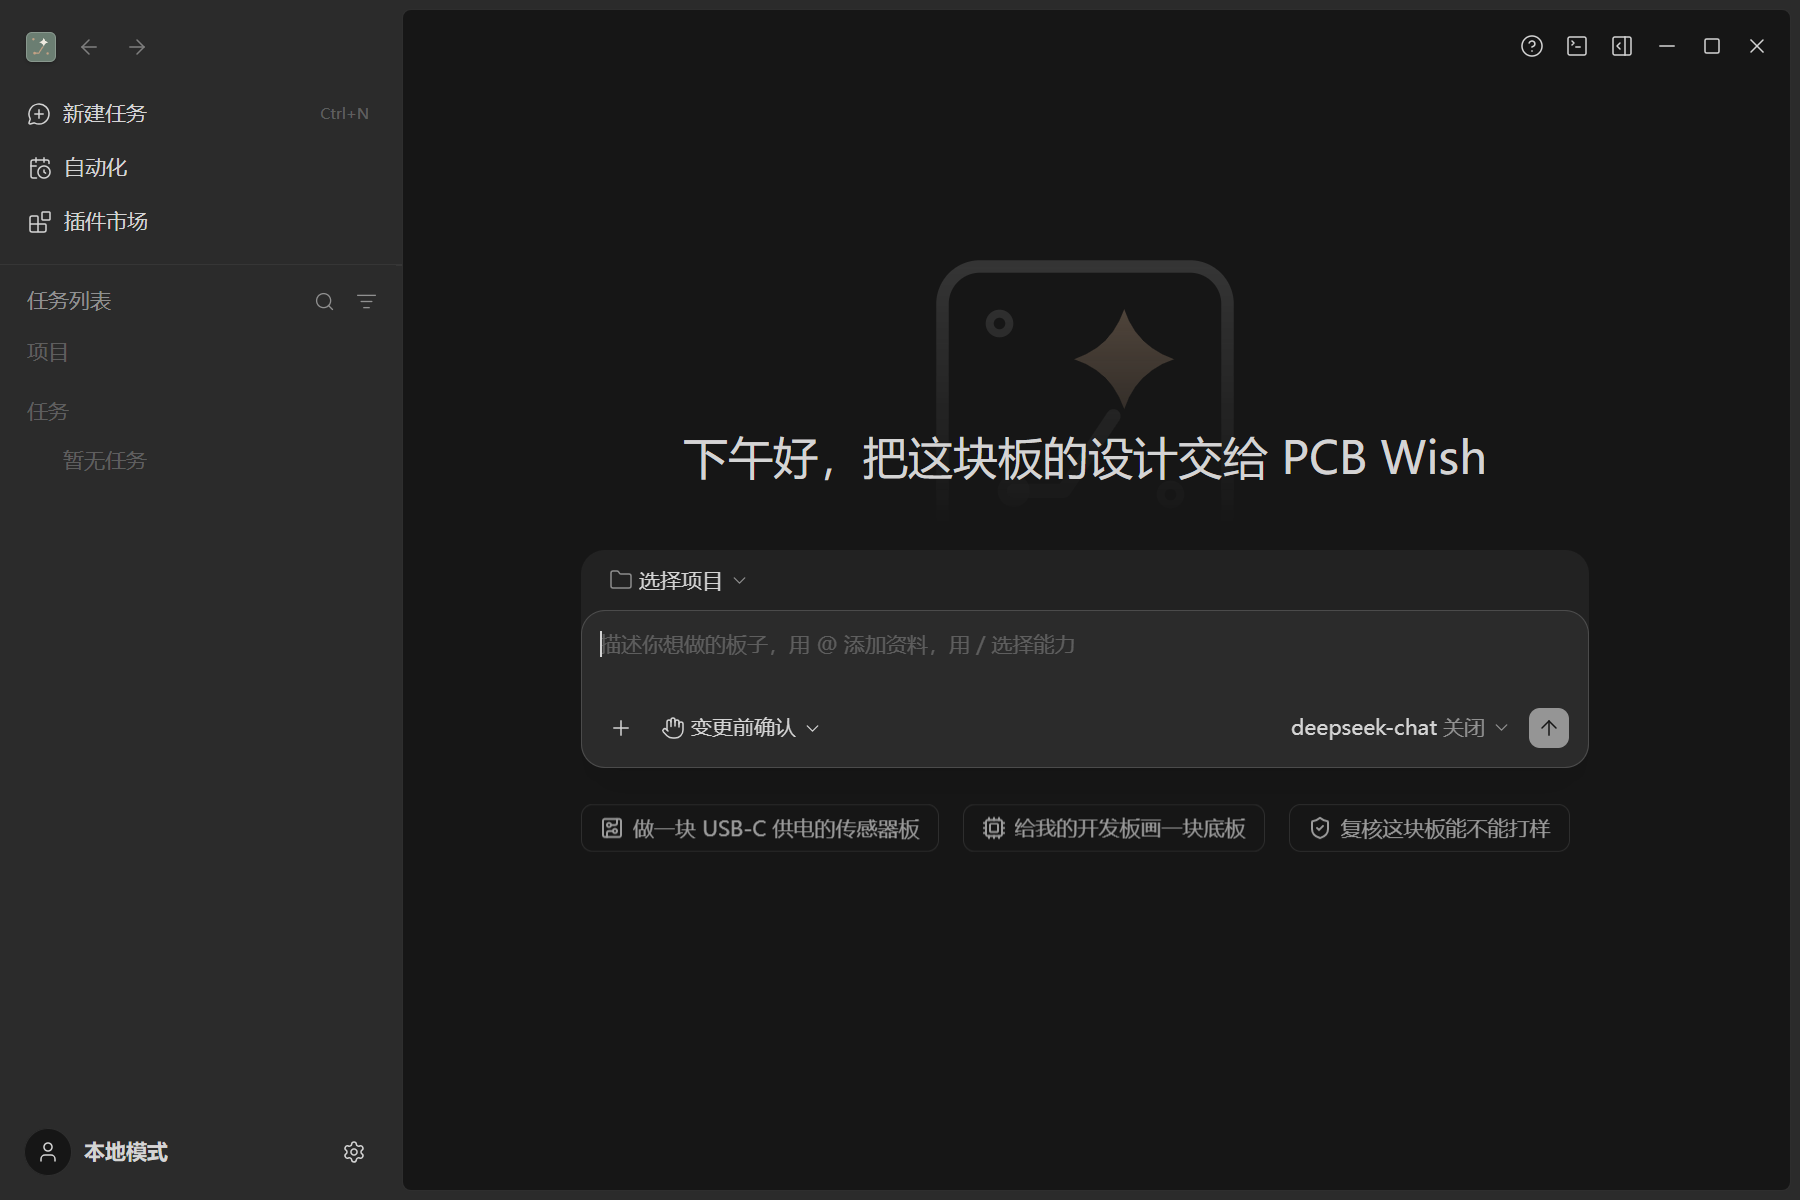
\includegraphics[width=0.96\textwidth]{app-home.png}}%
\endgroup
\caption{PCB-Wish 首页。选择工作区后，在输入框中描述板卡需求。}
\end{figure}

\subsection{第二步：描述需求}

使用日常语言描述板卡，建议覆盖以下六项：功能、供电、接口、尺寸与层数、焊接方式、打样渠道与成本。信息不完整时，系统会在受理阶段提问。完整示例见附录 A。

数据手册、旧原理图、板卡照片可直接拖入对话，或使用 \code{@} 添加。

\subsection{第三步：回答澄清问题}

受理角色会集中列出影响设计的缺口，最多两轮。用户可直接给出参数，也可选择“按你的建议来”，由系统给出默认方案并记录决策理由。缺口补齐后，系统进入设计阶段。

\subsection{第四步：执行设计}

设计开始后，系统按 G0 至 G7 逐门推进；每道门均以证据文件判定，未通过时系统会修正或暂停并提问。

\begin{itemize}
  \item 系统自动启动嘉立创EDA客户端，用户无需手动打开。
  \item 保存工程等少数操作需用户在客户端完成。
  \item 中等复杂度板卡通常需要数小时至数十小时，运行期间请保持窗口开启。
\end{itemize}

\begin{figure}[htbp]
\centering
\begingroup\setlength{\fboxsep}{0.8pt}%
\fcolorbox{line}{white}{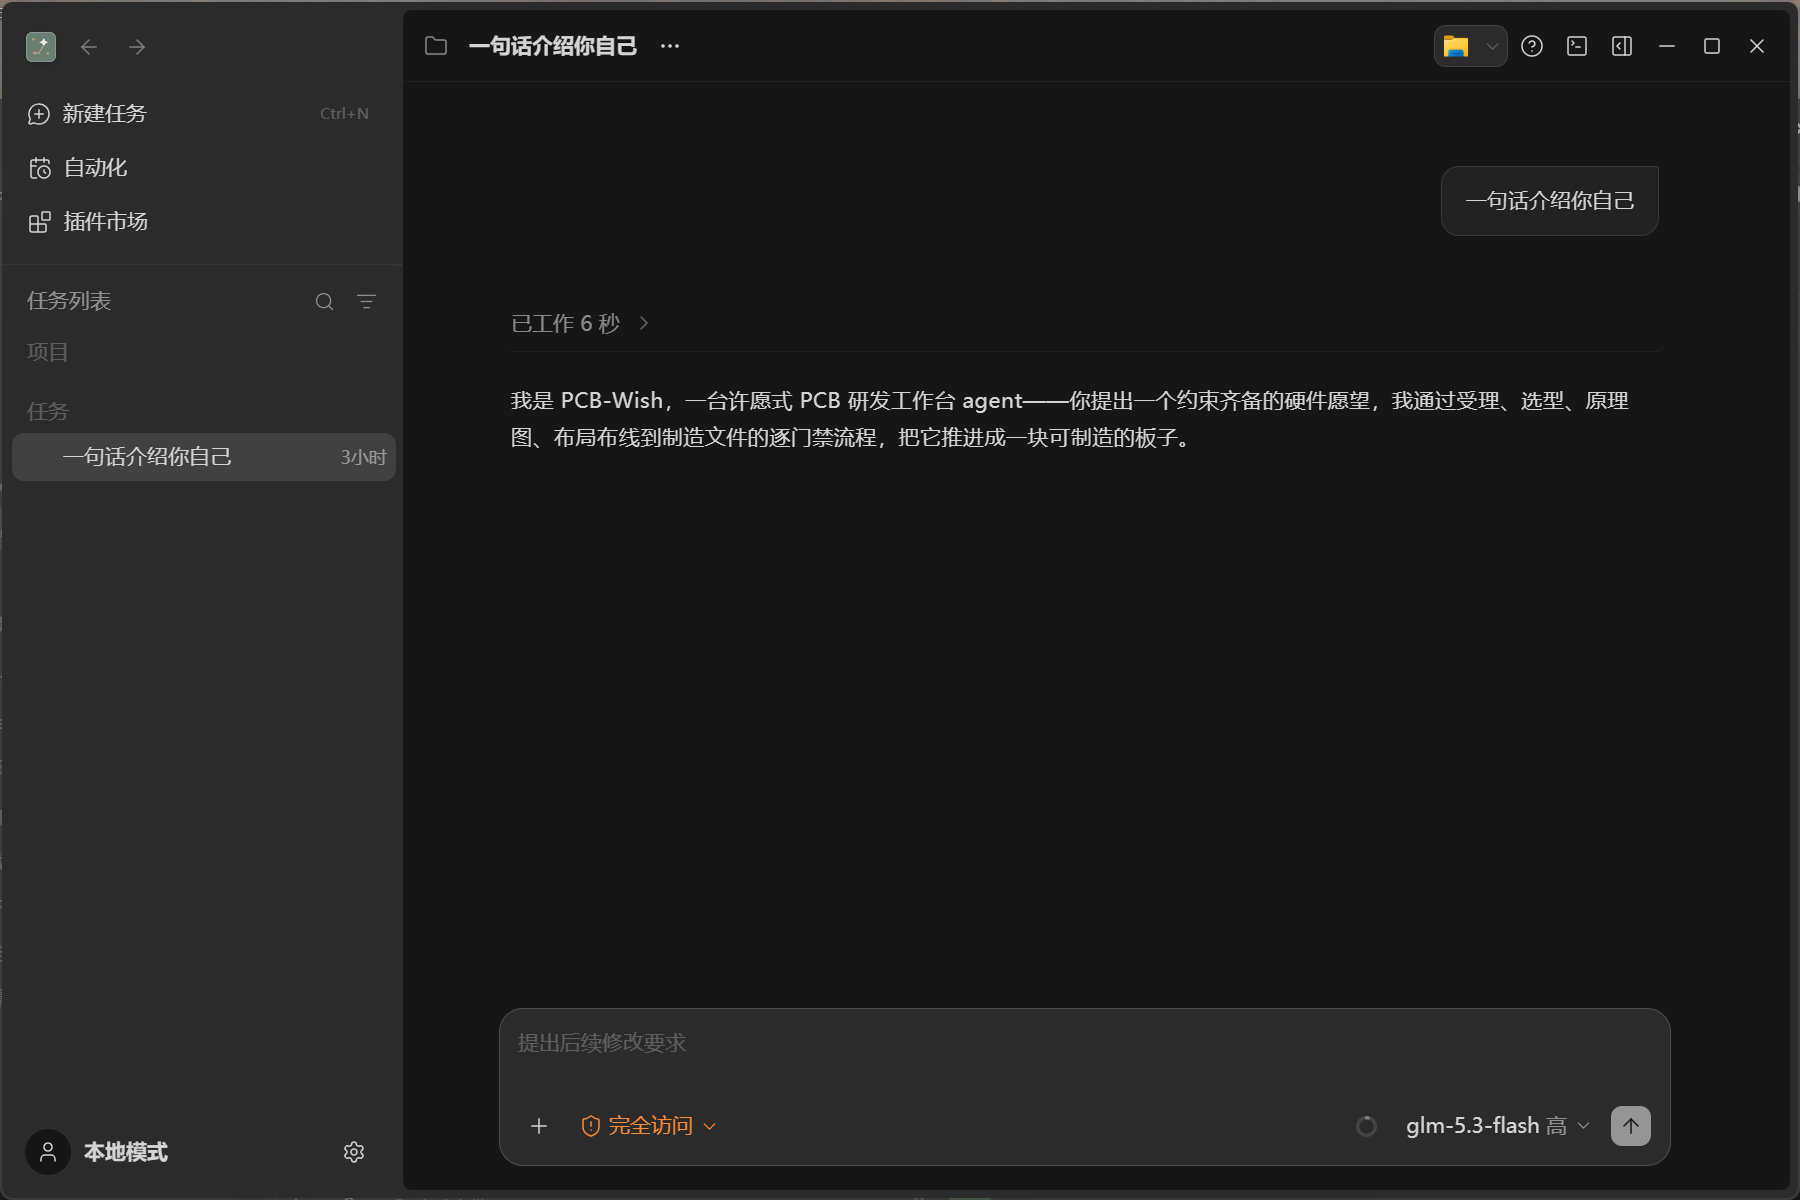
\includegraphics[width=0.92\textwidth]{app-conversation.png}}%
\endgroup
\caption{PCB-Wish 桌面版对话界面：左侧为任务入口，右侧为自然语言输入、智能体回复与模型选择。}
\end{figure}

\subsection{第五步：检查并接收交付物}

\begin{center}
\small
\begin{tabularx}{\linewidth}{@{}>{\RaggedRight\arraybackslash}p{6.3cm} >{\RaggedRight\arraybackslash}X@{}}
\toprule
\rowcolor{okbg}路径 & 内容 \\
\midrule
projects/<slug>/MISSION.md & 需求说明书与验收清单 \\
projects/<slug>/spec/ & 设计意图、BOM、检查清单 \\
projects/<slug>/reports/ & 检查报告、装配说明、交付说明 \\
projects/<slug>/export/gerber/ & Gerber 与钻孔文件，用于打样 \\
projects/<slug>/export/assembly/ & BOM 与贴片坐标 \\
projects/<slug>/teaching/lecture.pdf & 教学讲义（用户明确要求后生成） \\
\bottomrule
\end{tabularx}
\end{center}

% ==================== 6 ====================
\section{系统工作流程}

系统按“需求 $\to$ 受理与选型 $\to$ 设计 $\to$ 独立质检 $\to$ 交付”的主线推进；教学讲义为按需分支，仅在用户显式要求讲义的项目中执行。每个阶段设置门禁，未通过不得进入下一阶段。

\begin{figure}[htbp]
\centering
\begin{tikzpicture}[
  box/.style={draw=line,fill=cream,rounded corners=1.5mm,align=center,
    inner sep=2.2mm,minimum height=1.45cm,text width=2.45cm,font=\footnotesize},
  arrow/.style={-{Stealth[length=2mm]},thick,draw=sage}
]
\node[box] (n1) {需求\\（自然语言）};
\node[box,right=4mm of n1] (n2) {受理 + 选型\\G0 / G0.5};
\node[box,right=4mm of n2] (n3) {设计\\G1--G5.5};
\node[box,right=4mm of n3] (n4) {独立质检\\G6};
\node[box,right=4mm of n4] (n5) {交付\\文件 + 报告};
\draw[arrow] (n1) -- (n2);
\draw[arrow] (n2) -- (n3);
\draw[arrow] (n3) -- (n4);
\draw[arrow] (n4) -- (n5);
\node[box,below=7mm of n5,dashed] (n6) {教学讲义\\G7（按需）};
\draw[arrow,dashed] (n5) -- (n6);
\end{tikzpicture}
\caption{系统主线流程。教学讲义为按需分支。}
\end{figure}

\begin{figure}[htbp]
\centering
\begingroup\setlength{\fboxsep}{0.8pt}%
\fcolorbox{line}{white}{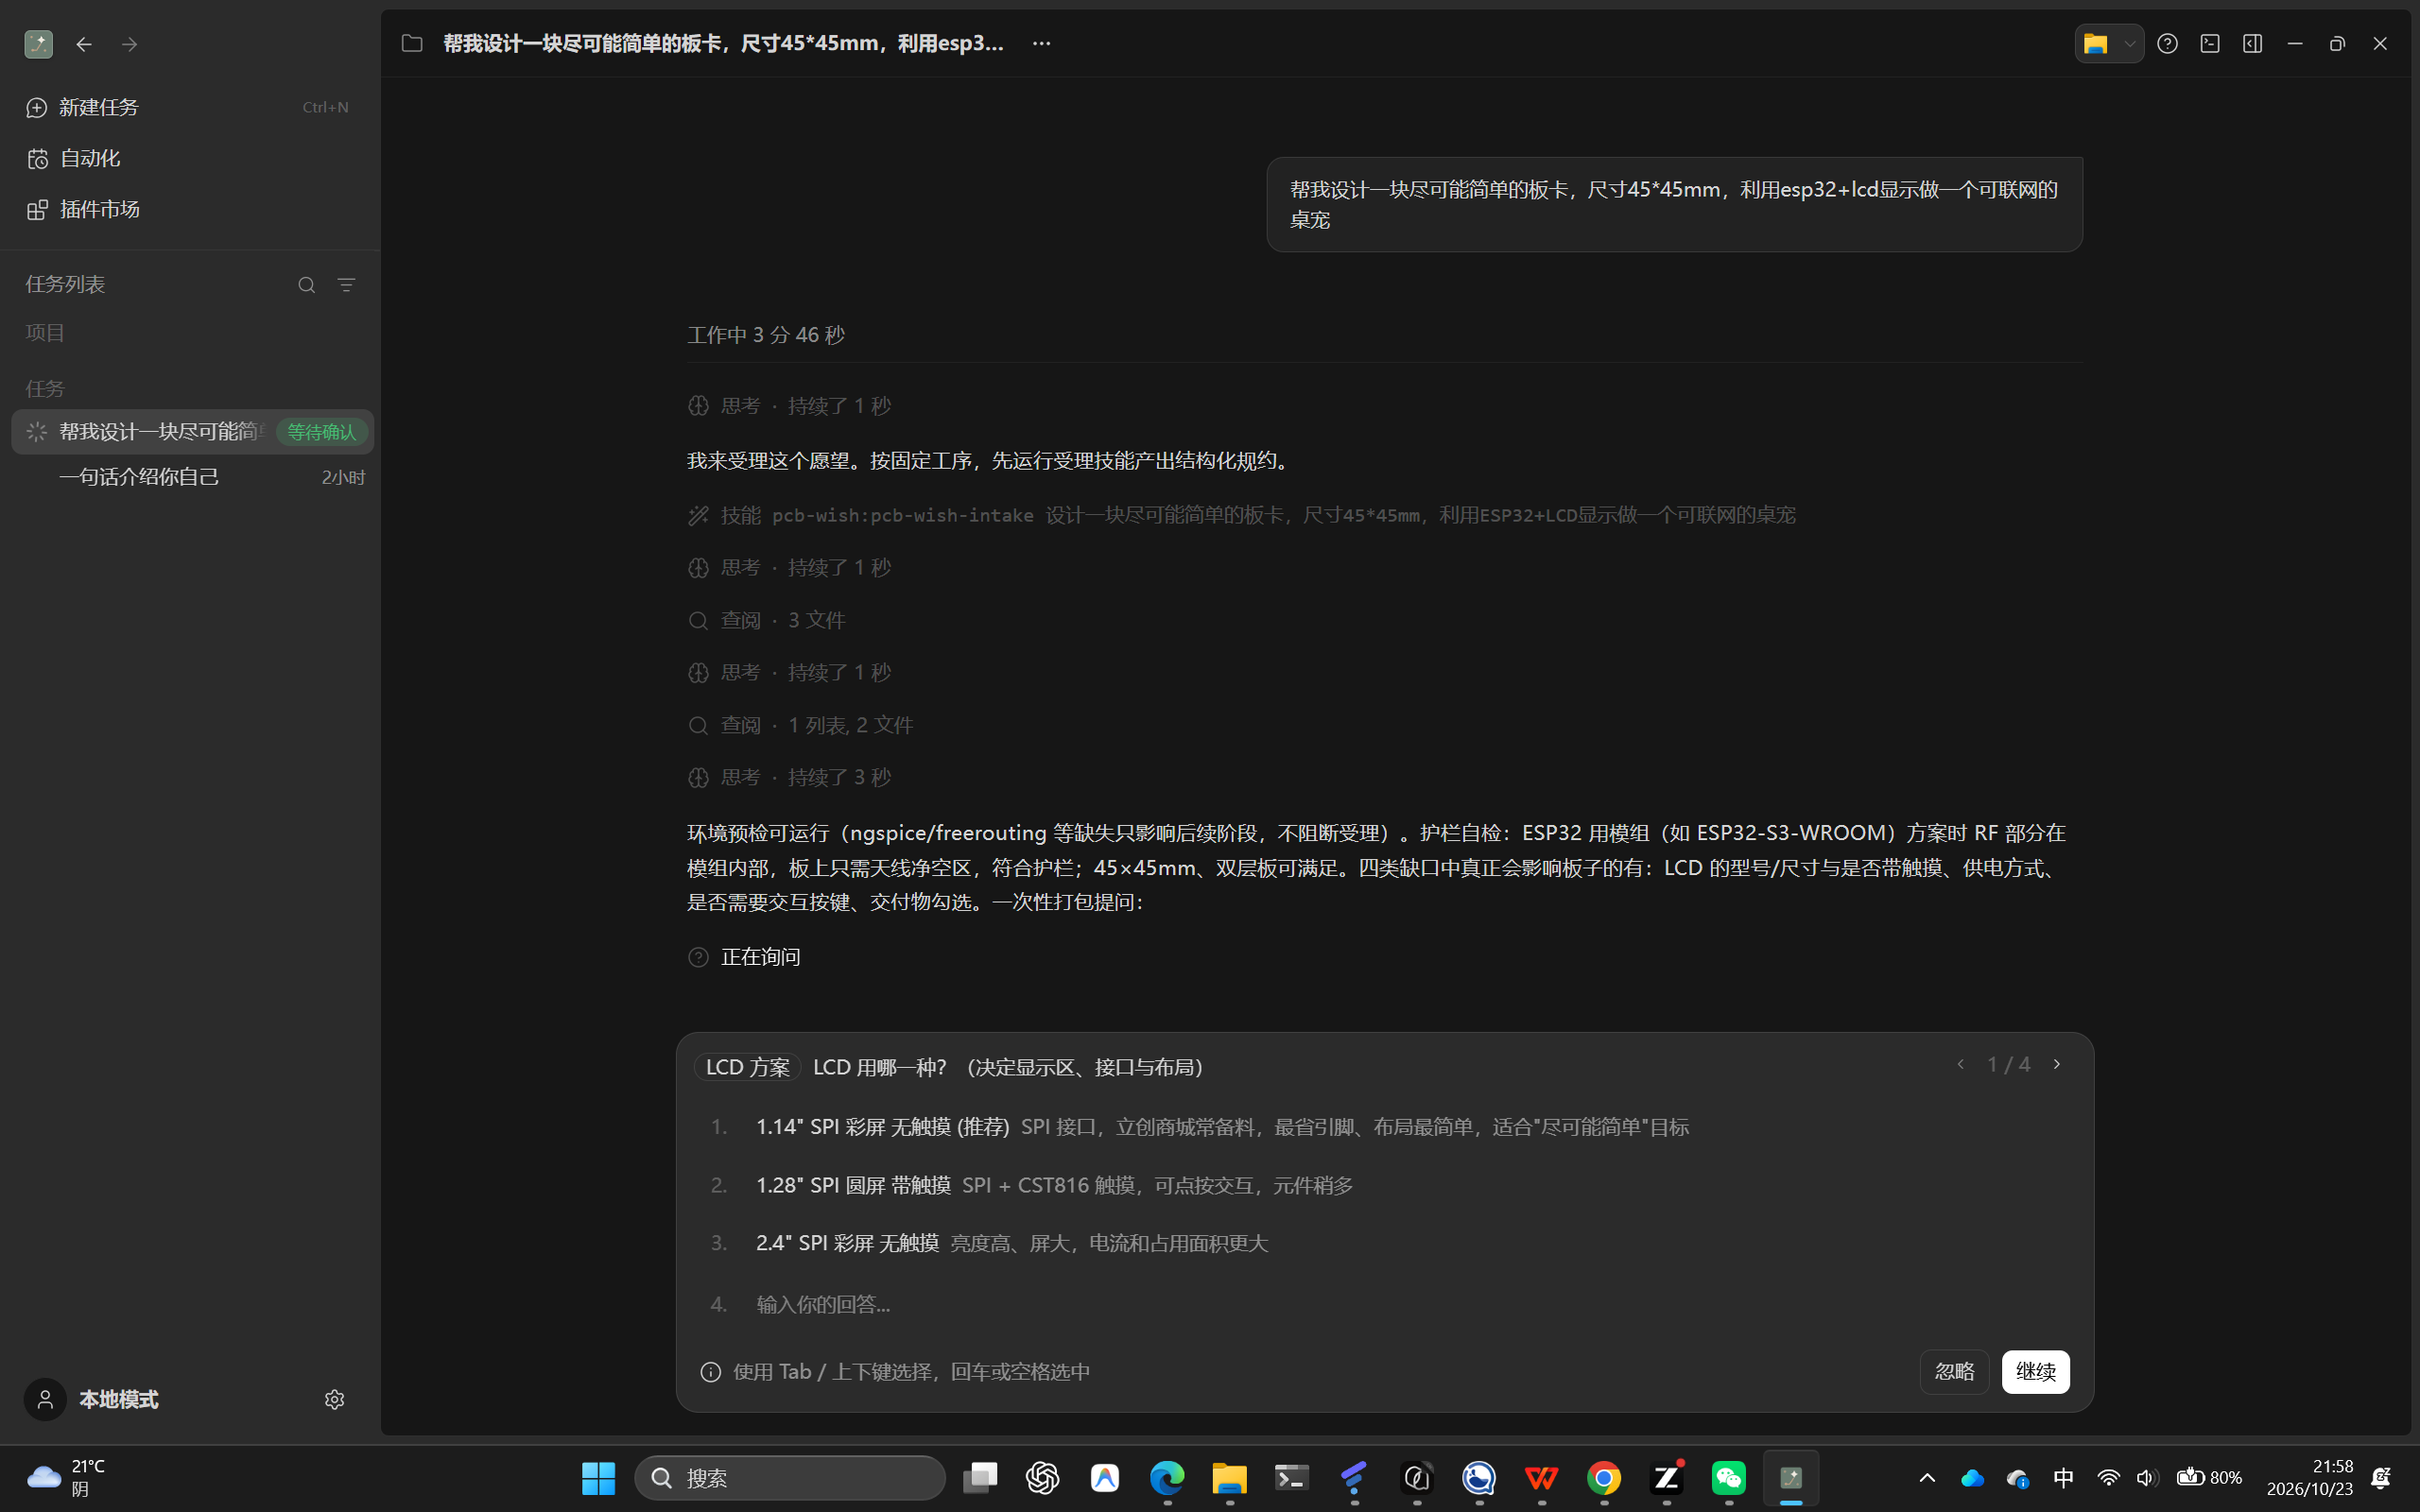
\includegraphics[width=0.88\textwidth]{app-workflow.png}}%
\endgroup
\caption{PCB-Wish 实际运行状态：受理实际板卡需求后进入澄清流程，任务已创建、技能已加载，系统正在集中提问。}
\end{figure}

\subsection{角色与产出}

\begin{center}
\small
\begin{tabularx}{\linewidth}{@{}>{\bfseries}p{2.7cm} >{\RaggedRight\arraybackslash}p{6.4cm} >{\RaggedRight\arraybackslash}X@{}}
\toprule
\rowcolor{okbg}角色 & 职责 & 主要产出 \\
\midrule
受理员 & 将需求整理为可验收规格；补齐影响设计的缺口 & \code{MISSION.md} \\
选型员 & 在嘉立创库中确定型号与封装，冻结 BOM & \code{spec/bom.json}、选型证据 \\
设计员 & 模块分解、标准块复用、驱动 EDA 完成原理图与 PCB & 原理图、PCB、布线、铺铜、丝印 \\
质检员 & 以只读方式独立复核 & 验收报告、PASS/FAIL 证据 \\
讲义作者 & 基于已验证工程生成讲义，数字需有出处 & LaTeX 源码、PDF、质检报告 \\
\bottomrule
\end{tabularx}
\end{center}

\subsection{阶段门禁}

\begin{center}
\small
\begin{tabularx}{\linewidth}{@{}>{\bfseries}p{1.4cm} >{\RaggedRight\arraybackslash}p{4.9cm} >{\RaggedRight\arraybackslash}X@{}}
\toprule
\rowcolor{okbg}门 & 名称 & 检查内容 \\
\midrule
G0 & 方案确认 & 功能目标与总体方案由用户确认 \\
G0.5 & 选型定稿 & 器件可采购、封装正确，BOM 冻结 \\
G1 & 设计意图 & 网络连接明确，检查清单与设计意图一致 \\
G2 & 原理图 & 原理图完成，规则检查与网表检查通过 \\
G3 & PCB 规划 & 板框、层叠与功能分区确定 \\
G4 & 布局 & 器件无重叠，丝印与朝向满足可布性 \\
G5 & 布线 & DRC、连通性与拐角比例通过 \\
G5.5 & 清零 & 错误与警告清零，或逐条豁免并记录理由 \\
G6 & 制造 & Gerber、钻孔、BOM、坐标与 DFM 可交付 \\
G7 & 讲义 & LaTeX 编译成功（用户要求讲义后执行） \\
\bottomrule
\end{tabularx}
\end{center}

\subsection{复核机制}

\textbf{独立质检。}质检角色由独立智能体承担，仅以只读方式访问文件和运行检查。它重新读取画布、执行网表检查并解析 Gerber，不采用设计角色的口头结论。

\textbf{网表检查。}设计前先记录“必须连接”和“禁止连接”的引脚关系，布线后逐条比对。即使 DRC 为 0，同网短路或漏连仍可被识别。

\textbf{硬门禁。}每道门均要求证据文件。未通过 G4 的布线操作、未通过 G5.5 的制造文件导出会被系统拦截。门禁依据证据文件，不依据模型的口头判断。

系统复用已验证的电路块，减少重复设计。

% ==================== 7 ====================
\section{能力边界}

\subsection{测试范围与预算限制}

受预算限制，目前完成了一次完整的人工在环测试，即第 8 节的 FlexiHeal v2。测试过程中有人工回答提问、确认方案与验收结果；尚未进行完全无人干预的完整流程测试。本次测试仅使用该项目的任务书作为需求输入，不代表测试结果已交付或投入使用。

后续需要更多轮测试、更多预算与失败样本，才能验证连续无人值守运行。教学讲义目前仅展示默认技能包的产出，其他开源技能包的组合效果尚未展示，原因同样是预算限制。

\subsection{当前局限}

受当前通用大模型模态能力限制，以及开发过程中缺少专业电子工程师和相关领域教师的指导，本项目的效果尚不尽如人意。后续希望随着通用模型能力提升，或电子工程师通过 LoRA 等方式获得专精于电子设计的模型，并结合工程师对本项目的改进意见，使系统能够切实帮助学习电子设计的同学。

% ==================== 8 ====================
\section{测试案例：FlexiHeal v2}

FlexiHeal v2 是目前唯一一次从需求推进到制造文件、再生成教学讲义的完整测试。工程位于 \code{E:\textbackslash agent project\textbackslash projects\textbackslash flexiheal-v2}。

\subsection{任务}

设计一块柔性弯曲传感器角度测量板：将传感器 53--90\,$\Omega$ 的电阻变化转换为 0--3.3\,V 电压，送入主控的模数转换口（ADC）；支持 USB/锂电池供电与充电、OLED 接口、0$^\circ$/90$^\circ$ 校准按键和调试口；由委托方手工焊接。

\clearpage
\subsection{结果}

\begin{figure}[htbp]
\centering
\begingroup\setlength{\fboxsep}{0.8pt}%
\fcolorbox{line}{white}{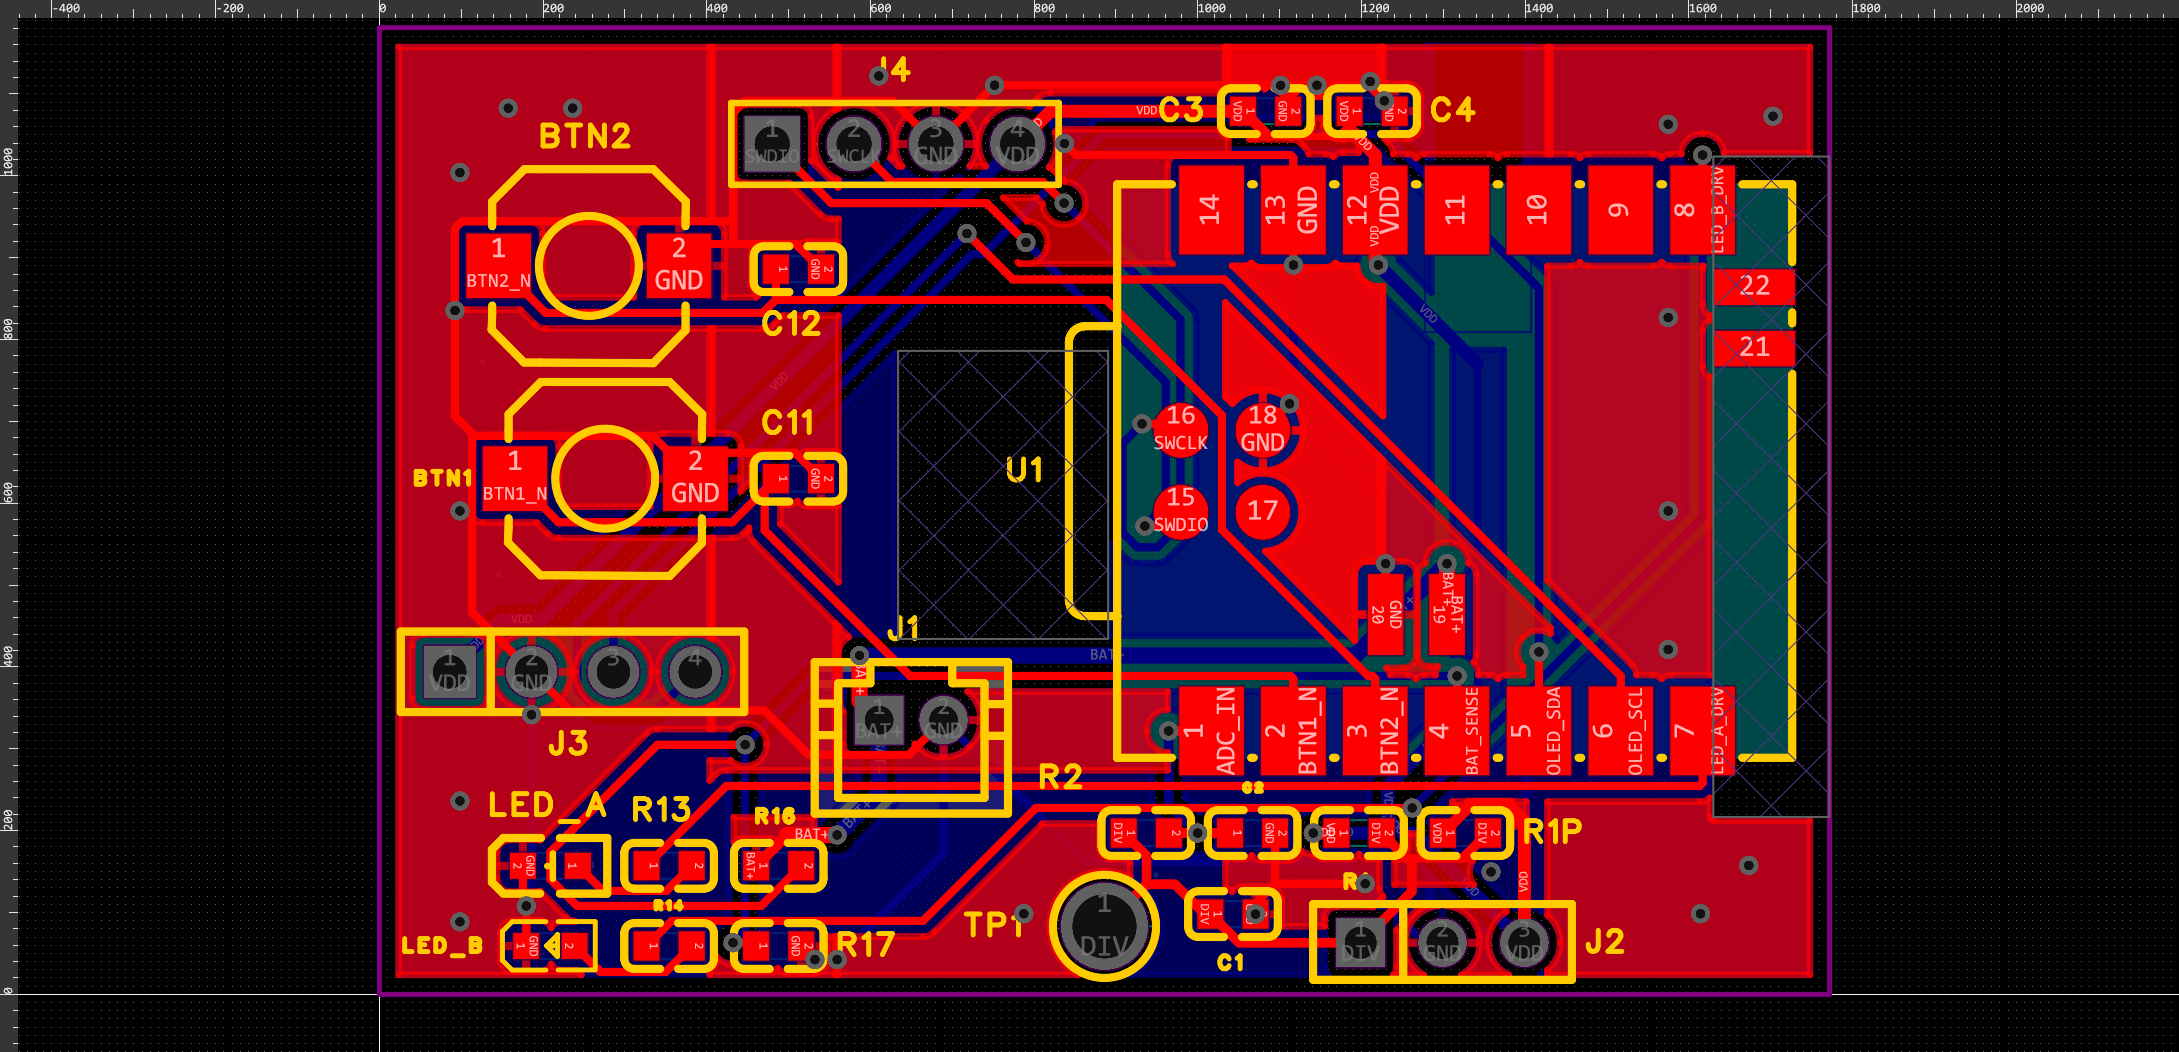
\includegraphics[width=0.95\textwidth]{board-pour.png}}%
\endgroup
\caption{FlexiHeal v2 顶层铺铜完成图（红：顶层铜；蓝：底层铜；黄：丝印与焊盘）。}
\end{figure}

\subsection{结论}

\begin{itemize}
  \item \textbf{完成实物工程交付。}Gerber、钻孔、BOM、贴片坐标、装配说明、检查报告与 58 页讲义均为实际工程产物，制造文件经过两路独立复核。
\end{itemize}

该案例验证了系统在中小规模板卡上的完整交付能力，同时暴露了判据、讲义质量与人工收尾方面的边界。

% ==================== 9 ====================
\section{教学讲义}

\subsection{讲义现状}

教学讲义不是默认交付物。只有用户在受理阶段用显式语言要求教学讲义，它才会进入 \code{MISSION.md} 的交付物清单。若无显式说明，受理智能体可能回问是否需要；未确认或未选择时不生成，并在交付说明中注明。用户要求讲义后，系统在板卡通过 G6 后生成 PDF。当前结构为 1 章总览加 7 个功能模块章；每章按“内容提要、工作原理、设计依据与计算、PCB 布局布线要点、验证方法与结果”五段展开，不包含习题与 PCB 通识附录。

FlexiHeal v2 讲义共 58 页、27 张真实工程图（原理图分区、板级截图、厂商引脚图），另有 10 处正文重绘；关键数字尽量对应到实测、计算或仿真记录，出处覆盖率 95.5\%。

\subsection{讲义局限}

讲义仍存在明显的 AI 生成痕迹：句式工整、结构趋同、案例偏模板，关键取舍的深度不足。使用时需提供课程大纲、课时与学生水平，并由教师逐页审阅与润色。

改进方式包括：提供课程大纲、课时与学生水平；提供实测值、仿真波形和失败案例；要求图表与数据注明来源；由教师完成最终审阅。

\begin{figure}[htbp]
\centering
\begingroup\setlength{\fboxsep}{0.8pt}%
\fcolorbox{line}{white}{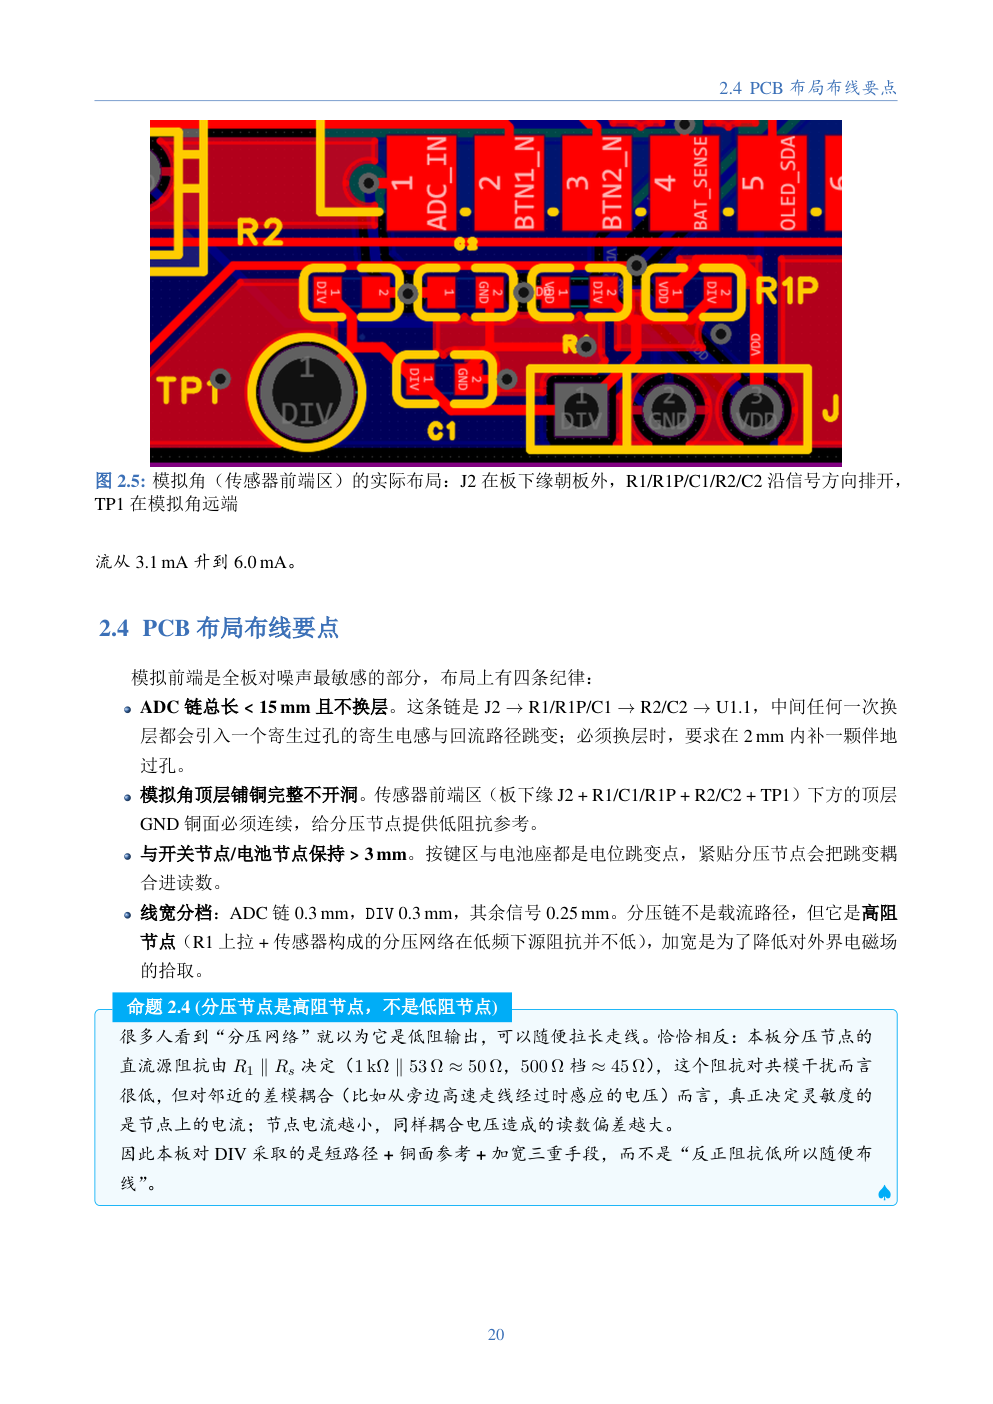
\includegraphics[width=0.72\textwidth]{lecture-sample.png}}%
\endgroup
\caption{FlexiHeal v2 讲义示例页：PCB 布局要点与工程实例图。}
\end{figure}

% ==================== 10 ====================
\section{发展方向}

\subsection{与其他开源技能包结合}

讲义生成是一个独立技能包，可与其他开源教学、绘图、排版技能包组合，分别负责插图、习题、排版与事实核查。相比单一模型从头生成，组合方式更接近教材编写流程。

\subsection{工具与流程改进}

\begin{itemize}
  \item 深化 EDA 接口，减少保存工程、导出 PDF 等人工操作；
  \item 引入约束驱动布线与成熟的自动布线器，减少反复补线；
  \item 将走线对齐、过孔整齐、丝印可读、器件朝向等美观指标量化，用评分驱动修改。
\end{itemize}

\begin{center}
\small
\begin{tabularx}{\linewidth}{@{}>{\bfseries}p{2.0cm} >{\RaggedRight\arraybackslash}X@{}}
\toprule
\rowcolor{okbg}阶段 & 目标 \\
\midrule
近期 & 完善环境自检与失败恢复；降低讲义 AI 痕迹；扩充标准块库 \\
中期 & 建立布局布线美观评分 \\
远期 & 打通需求到小批量交付的完整链路；教师少量修改即可授课；关键节点保留人工签字 \\
\bottomrule
\end{tabularx}
\end{center}

\subsection{人机分工}

系统承担重复查表、逐条比对、报告生成与排版工作；用户负责需求确认、关键取舍与最终验收。目标是减少重复劳动，同时保留工程判断与责任边界。

% ==================== 11 ====================
\section{附录 A：示例需求与预期输出}

\subsection{示例需求}

\begin{leadbox}
我想做一块 USB-C 供电的传感器转接板：3.3\,V 输出，带一个 I2C 接口和一个指示灯；两层板，板框 30\,mm $\times$ 20\,mm，嘉立创打样，成本尽量低，手工焊接。
\end{leadbox}

\subsection{预期行为}

\begin{enumerate}
  \item 解析已给出的功能、供电、接口、尺寸、工艺与成本约束；
  \item 列出影响设计的缺口，例如传感器型号、输出电流、接口针数与安装方式；
  \item 集中提问，最多两轮；用户可指定默认方案；
  \item 生成 \code{projects/<slug>/MISSION.md} 并执行完备性校验；
  \item 校验通过后进入选型与设计阶段；未通过则暂停并等待补充。
\end{enumerate}

\subsection{预期输出}

\begin{center}
\small
\begin{tabularx}{\linewidth}{@{}>{\RaggedRight\arraybackslash}p{6.3cm} >{\RaggedRight\arraybackslash}X@{}}
\toprule
\rowcolor{okbg}输出 & 内容 \\
\midrule
MISSION.md & 功能、约束、验收清单与授权状态 \\
spec/ & 设计意图、BOM、检查清单 \\
reports/ & 门禁记录、检查报告、装配说明、交付说明 \\
export/gerber/ & Gerber 与钻孔文件 \\
export/assembly/ & BOM 与贴片坐标 \\
teaching/lecture.pdf & 讲义（用户明确要求后生成） \\
\bottomrule
\end{tabularx}
\end{center}

实际提问与输出随需求缺口变化；示例仅用于说明流程。

% ==================== 12 ====================
\section{致谢}

本项目使用了多项开源软件与开放工具。主要项目如下，完整依赖见仓库的 \code{package.json}、\code{pnpm-lock.yaml} 与 \code{THIRD-PARTY-NOTICES.md}。

\subsection{上游与桌面端}

\begin{itemize}
  \item \textbf{ZCode}（\code{zai-org/ZCode}，Apache-2.0）：本仓库上游开源框架；PCB-Wish 在此基础上做任务特化修改，并沿用它提供的桌面应用、智能体命令行、运行时与基础设施。
  \item \textbf{Electron}、\textbf{Node.js}、\textbf{React}、\textbf{TypeScript}、\textbf{Vite}、\textbf{pnpm}、\textbf{Vitest}、\textbf{Zustand}：桌面端与开发工具链。
\end{itemize}

\subsection{PCB 与 EDA}

\begin{itemize}
  \item \textbf{嘉立创EDA专业版}：提供客户端、命令行与接口通道，是设计执行的基础。
  \item \textbf{easyeda-agent}（MIT，部分组件 Apache-2.0）：早期驱动层与 EDA 接口封装参考。
  \item \textbf{ngspice}（GPL）：电路仿真。
  \item \textbf{FreeRouting}：密集板自动布线增强。
  \item \textbf{KiCad}（GPL-3.0）及 \code{kicad-cli}：第二套 EDA 工具，用于交叉检查。
  \item \textbf{spicelib}（GPL-3.0）：网表与仿真文件解析。
  \item \textbf{CircuitJS1}（GPL-2.0+）：引用在线服务，未修改、未分发其代码。
\end{itemize}

\subsection{讲义与排版}

\begin{itemize}
  \item \textbf{TeX Live / MiKTeX}、\textbf{XeLaTeX}：讲义编译。
  \item \textbf{ctex}、\textbf{ElegantBook}、\textbf{TikZ/PGF}、\textbf{circuitikz}、\textbf{tcolorbox}、\textbf{booktabs}、\textbf{caption}、\textbf{hyperref}、\textbf{enumitem}（LPPL 或兼容许可）：中文排版、图示、表格与文本盒。
\end{itemize}

\subsection{质量与文档}

\begin{itemize}
  \item \textbf{Python} 及其标准库：插件脚本、门禁与检查工具。
  \item \textbf{pypdf}（BSD-3-Clause）：PDF 文本层与页面检查。
  \item \textbf{PyMuPDF}（AGPL-3.0）：讲义逐页视觉检查。
  \item \textbf{matplotlib}（Matplotlib License）：仿真与数据图。
\end{itemize}

桌面端第一方代码沿用上游 Apache-2.0；PCB-Wish 插件为 MIT；第三方组件遵循各自许可。

\subsection{特别感谢}

感谢 FlexiHeal 项目的委托方提供真实任务书、验收意见与修改建议；这些意见直接推动了讲义与流程的改进。

受限于时间和经费，当前项目仍处在“半成品”阶段，还有很多可改进的地方。但我衷心希望该项目可以切实帮助到学习电子设计的同学们（包括我）。后续如有机会，希望可以进一步改进该项目。

\vspace{1.2em}
{\small\color{ink2} 本文档使用 XeLaTeX 排版。源码：\code{README.tex}；图片：\code{docs/readme/images/}。}

\end{document}
